%\documentclass[aps,pra,reprint,longbibliography]{revtex4-1}
\documentclass[twocolumn]{article}

\usepackage{geometry}
\geometry{textwidth = 18cm,textheight = 24cm}

%\usepackage{multicol}
\usepackage{caption}

\usepackage{graphicx}
\usepackage{amsmath}
\usepackage{float}
%\usepackage{amssymb}
\usepackage{textcomp}
%\usepackage{lmodern}
\newenvironment{figure_alt}
  {\par\medskip\noindent\minipage{\linewidth}}
  {\endminipage\par\medskip}

\begin{document}
	
	%-------------------- begin header -------------------%
	\centerline{\LARGE Optoelectronic Intelligence}%Light in neural systems%Intelligent optoelectronic systems
	\vspace{0.75em}
	\centerline{\Large Jeffrey M. Shainline}
	%\vspace{0.75em}
	%\centerline{\large National Institute of Standards and Technology}
	\vspace{0.5em}
	\centerline{\large NIST, Boulder, CO, 80305}
	\vspace{0.5em}
	\centerline{\large \today}
	%-------------------- end header ---------------------%
	
\begin{abstract}

\end{abstract}

\section{\label{sec:introduction}Introduction}
Light is excellent for communication. Fiber optic links carry vast quantities of information across continents and between data centers. An important question in modern computing is: what is the shortest distance over which photonic communication will displace electronic interconnects? Optical links between racks in data centers are becoming common \cite{}. Major companies are investing seriously in photonics in the package. Monolithic optical links between processor and memory fabricated in a 45-nm CMOS node with no in-line changes have been demonstrated \cite{suwa2015}. A primary challenge affecting further chip-scale electronic-photonic integration is the continued difficulty of achieving a light source implemented on silicon that is robust, efficient, and economical.

In parallel with the hardware considerations affecting optoelectronic integration are questions related to architecture. A prominent theme emerging since clock speed leveled off in 2003 \cite{} is parallelism. Computation is increasingly distributed among more processor cores. Many-core architectures continue to expand into on-chip networks, in some cases resulting in highly distributed, brain-inspired systems \cite{}. As compute grows more distributed, communication across interconnection networks becomes a bottleneck. The demand for energy efficient communication bandwidth has been a major driver of on-chip photonics.

The major drivers for brain-inspired computers fall on a spectrum: energy and algorithmic efficiency for deployable applications reside on one side of the spectrum, and artificial general intelligence (AGI) resides on the other. Knowledge gained from neuroscience informs us that systems with general intelligence will benefit from very large numbers of computational elements as well as extreme communication between them. It is our perspective that hardware incorporating light for communication between electronic computational elements combined with an architecture of distributed optoelectronic spiking neurons will provide tremendous potential for AGI. Considerations pertinent to the realization of such a technology are the subject of this article.

\section{\label{sec:neuroFractalsAndVLSI}Neuroscience, fractal geometry, and very-large-scale integration}
\begin{figure*} 
    \centering{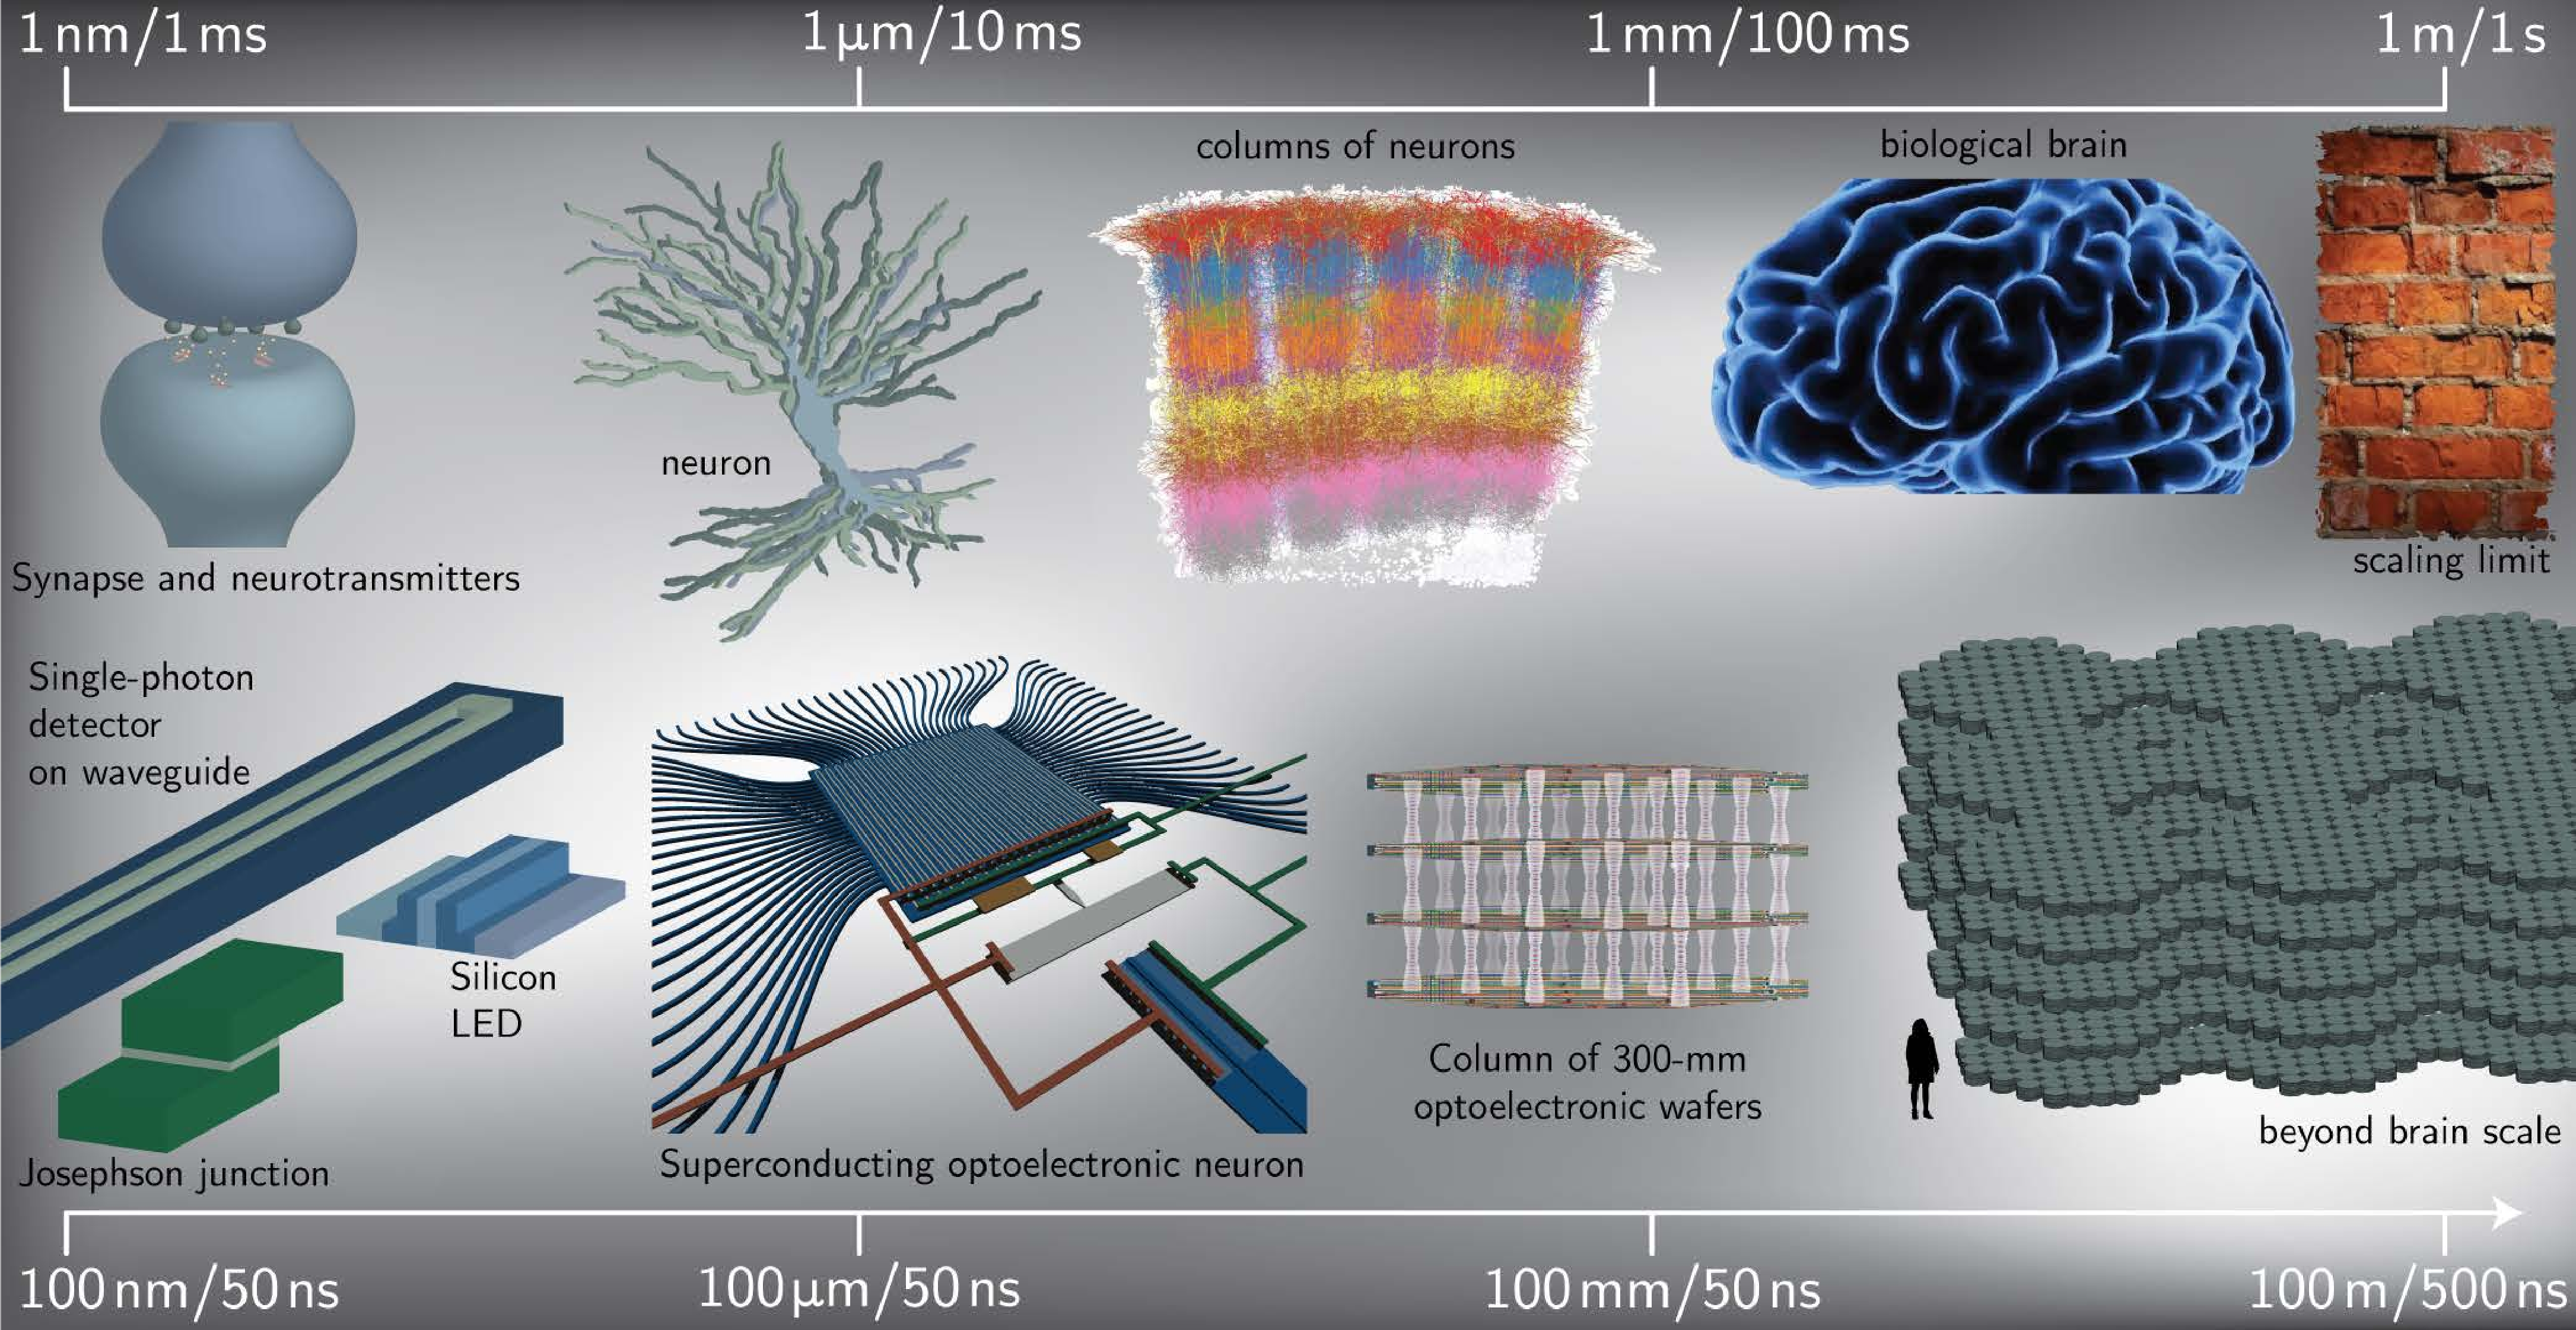
\includegraphics[width=17.2cm]{complexity_across_scales.pdf}}
	\captionof{figure}{\label{fig:complexityAcrossScales}Complexity across scales.}
\end{figure*}
To guide the design of hardware for AGI, we must simultaneously consider the principles of neural information and very-large-scale integration (VLSI). Both lead to fractal scaling.

Information processing in neural systems employs local clusters of neurons to represent specific features, and the information from these clusters must be shared with other regions of the network to form a multifaceted representation of a complex stimulus. The dynamical patterns of activity that accomplish this information integration are neuronal avalanches, cascades of spiking activity across local, regional, and global partitions of the network. We denote by $s$ the number neurons involved in a neuronal avalanche. Brain activity across many species, brain regions, and contexts shows the probability of observing an avalanche of size $s$ follows a power law: $P(s)\sim s^{-\alpha}$. Systems with a power-law distribution of neuronal avalanches demonstrate self-organized criticality \cite{}, which maximizes the dynamic range of the system \cite{}. Such a power-law dependence has the important property that the ratio of number of events of size $qs$ to the number of events of size $s$ is simply $q^{-\alpha}$, independent of $s$. For this reason, such a distribution is referred to as ``scale-free'', and is self-similar, or fractal, across spatial and temporal scales. 

Fractal properties of neural systems are crucial to their operation. Fractal systems can continue to scale, with dynamics constrained only by the physical hardware and spatial extent of the system rather than by the ability to communicate across the architecture \cite{plth2007}. Such scale-free systems can efficiently integrate information from local clusters to vast networks, while enabling correlations across wide regions of space and long periods of time. 

Achieving the necessary communication for scale-free systems across space and time places severe demands on hardware. The physical requirements for supporting neuronal avalanches across a broad range of scales can be understood from the perspective of Rentian scaling, first explored in the context of VLSI microelectronic circuits \cite{}. Rentian analysis tracks the relationship between the number of nodes within a volume of space and the number of connections emanating from that volume for partitions of the network from a single node to the network as a whole. It has been observed empirically that a wide variety of systems from electronic processors to biological neural networks obey a relationship of the form $e_i\sim n_i^{\beta}$, where $e_i$ is the number of edges emanating from the $i$th hierarchical partition of the network, $n_i$ is the number of nodes confined within that partition, and $\beta$ is referred to as the Rent exponent. Again, a scale-free relation is found. To best achieve Rentian scaling across very large systems, and thereby enable large neuronal avalanches, optical communication infrastructure is necessary.  

The dynamical attributes of the network that give rise to neuronal activity across spatial and temporal scales must also be considered. The synaptic connections between neurons play a crucial role in enabling complex, dynamic activity. Short-term synaptic plasticity enables synapses to rapidly adapt in response to network activity, essentially resulting in temporal filtering of afferent spike trains \cite{abre2004}. Learning in the presence of a continually changing environment while maintaining long-term memories is achieved through spike-timing-dependent plasticity (STDP) \cite{somi2000} and metaplasticity \cite{ab2008}. Dendritic processing, wherein the dendritic arbor performs intermediate, nonlinear transformations between synapses and the soma, enables utilization of timing information \cite{vagu2005}, detection of sequences of activity \cite{haah2015}, and in conjunction with inhibitory interneurons enables specific inputs to be silenced or augmented at specific times \cite{bu2006}. A combination of excitatory and inhibitory neurons with complex plasticity mechanisms and dendritic processing allows a given structural network to implement a wide variety of dynamical functions, and allows efficient access to and integration of information across broad spatial and temporal scales. Dynamical electronic neurons and synapses can rapidly adapt the vast structural network enabled by photonic communication into myriad functional networks.  

This brief foray brings a few key messages relevant to the design of artificial neural hardware. Diverse activity across spatial and temporal scales requires a vast structural interconnection network with communication across spatial scales, as captured by Rentian scaling. We conjecture that light is most capable of achieving communication in complex neural systems, from the scale of local clusters to the entirety of an AGI. But neural activity also requires components adapting at various frequencies to enable myriad functional networks, as demonstrated by neuronal avalanches with activity at various frequencies, enabled by complex, adaptive synapses and dendrites. Such complex, adaptive activity is much better suited to the domain of electronic circuitry. Based on these consideration, we expect a hardware platform capable of AGI to combine the strengths of photonic communication with electronic computation to integrate information in neuronal avalanches from small, local clusters on a silicon wafer to the light-cone-limited region of space across which light can travel in a network oscillation cycle. 

\section{\label{sec:synapsesDendritesAndNeurons}Optoelectronic synapses, dendrites, and neurons}
The device factors mentioned above are not quirks of the biological world, but rather are some of the reasons brain computation is so complex and efficient. Short-term plasticity produces information about spike train rising and falling edges and guards against runaway activity. STDP strengthens correlations between neurons that fire constructively and dampens connections that waste energy. These mechanisms have been shown to adapt random structural networks into complex functional networks with small-world architecture and neuronal avalanches indicating maximal dynamic range due to criticality. Dendritic processing in conjunction with inhibitory interneurons makes efficient use of the complex spatial network by dynamically activating a wide range of functional networks. To achieve these myriad computational functions, optical interactions are inadequate. The complexity of electronic circuits is required. 

We envision optoelectronic hardware with communication along photonic axons, and computation performed in electronic synapses, dendrites, and neurons. We make two more choices to specify the platform. Detectors must respond to single photons for maximal energy efficiency. Superconducting-nanowire single-photon detectors (SNSPDs) are the clear choice for this application, with very low dark counts, near-zero static power dissipation, and scalable integration \cite{shbu2017b}. An SNSPD is simply a current-biased strip of superconducting wire roughly 100\,nm in width and 5\,nm in thickness. SNSPD operation is summarized as follows. In the steady state, the current bias flows straight to ground, and upon detection of a photon, a small section of the wire is driven from the superconducting phase to the normal-metal phase, resulting in a transient resistance of a few kilo-ohms for a few hundred picoseconds. This resistance produces a transient current bias a load. 

In addition to the choice of SNSPDs as the detectors in the system, we must also identify the most promising light source, which must be fabricated across wafers by the millions for economical, brain-scale systems. Because our choice of detectors dictates cryogenic operation, silicon light sources operating at 4\,K are an option \cite{da1989,shxu2007}. This neural system may be one of the few applications where silicon light sources are appropriate and sufficient. The light sources we have in mind are silicon LEDs, employing luminescence from defect-based dipole emitters \cite{buch2017}. From the perspective of VLSI, achievement of a silicon light source of sufficient performance would be the greatest contribution to the success of this technology.

To achieve complex neural circuits, we must combine light sources, detectors, and various other circuit elements. We have demonstrated waveguide coupling of light from these micron-scale light sources to integrated SNSPDs on a silicon photonic chip \cite{buch2017}. The detectors can be engineered in circuits with Josephson junctions (JJs) and superconducting loops coupled through mutual inductors to achieve the complex circuit functions we need for neural information processing. The current bias across a single JJ establishes the synaptic weight. This current bias can be modified through various photonic and electronic means based on network activity. Inhibition is straightforward with opposing mutual inductors. Dendritic and neuronal nonlinearities are a natural consequence of phase slips across JJs driven above their critical current, and the extreme nonlinearity of the superconducting phase transition playing a leading role, both for the detection of light at synapses and for the production of sufficient voltage to generate light during neuronal firing events. Due to the prominent role of superconducting current storage loops, we refer to these as loop neurons. In the operation of loop neurons, a single photon triggers a synaptic event, and STDP is induced by two photons\textemdash one from each neuron associated with the synapse. %Such hardware appears promising to achieve extreme communication across vast networks while maintaining very low power density, and reasonable system power consumption.

\section{\label{sec:communication}Communication with guided light}
The central premise of our work is that photonic signals are superior to electronic signals for communication across large-scale neural systems. To explain why we place this conjecture at the center of hardware development, we briefly summarize the physical limitations of electrical interconnection networks \cite{hepa2012}. It is impracticable in silicon electronics for a single device to source current to many other devices, so in practice a shared communication network is employed \cite{}. In contemporary computing, switched media networks are used for this purpose. Each device must then only communicate to the nearest switch in the network. The interconnect network determines a valid route for the information to traverse across the network, and the switches are configured accordingly. Because the communication infrastructure is shared, devices must request access to the switch network to transmit messages. When multiple devices request access simultaneously, arbitration must be performed, wherein devices are queued and sequentially granted access to the switch network. This approach to communication between electronic devices leverages the speed of electronic circuits to compensate for the difficulties in communication. The limitations are reached when many devices need to communicate with many other devices with a high frequency of communication events. Unfortunately, this is exactly the situation encountered in neural information processing. During a neuronal avalanche, many neurons may need to communicate simultaneously across the network. As more neurons, each with many synapses, are added to the network, the average frequency of neuronal firing events must decrease due to the limitations of the interconnection network to handle communication requests, and large neuronal avalanches integrating information across the network cannot be supported by the communication infrastructure. %For electronic systems with a few hundred thousand neurons, average event rates in the kilohertz range can be maintained \cite{}. Systems with a few hundred million neurons will likely be limited to operation at 10 Hz or below \cite{}.

The requirement of utilizing a shared communication infrastructure results from the physics of electrons. Because electrons interact with each other due to their charge, they can be used to establish a voltage on a capacitor, which is useful for computing. But the charge-based interaction is also what makes it difficult to source sufficient current to directly communicate between many devices. The physics of light is complimentary to that of electrons. Photons, being uncharged bosons, interact with one another only through quantum interference, such as the Hong-Ou-Mandel effect. Light-matter interaction is generally weak, especially at low light levels. Thus, photons can co-propagate on waveguides independently of one another without wiring capacitance. This enables a pulse of photons to fan out to many destinations without a charging penalty due to wiring. This is not to say photonic communication can address an arbitrarily large number of recipients without consequence. For each new recipient, the number of photons in the initial pulse must increase, and as destinations get further away, more energy is dissipated to propagation loss. These realities notwithstanding, it appears feasible for devices communicating with photons to make direct, physical, point-to-point connections to many thousands of destinations, thereby eliminating the need for the shared communication infrastructure that is the primary impediment to achieving AGI with electrical interconnections.

Having made this claim, the burden is upon us to provide evidence of the feasibility of photonic communication in large-scale neural systems. Much like electrical interconnection networks utilize different technologies at the scales of chips versus data centers, photonic interconnection technologies must enable communication from the scale of an on-chip network to a many-wafer system the size of a data center. Further, the specific architectures suitable for neural information processing require that neurons be capable of communicating seamlessly across all scales of this network hierarchy. At the outset, the large wavelength of light relative to the size of electronic devices (and relative to the size of devices in the brain) give us concern for the size of brain-scale networks. To build confidence for the feasibility of the endeavor, we sketch a vision of how a general optoelectronic neural system may be constructed.

A successful neural technology must leverage the fabrication infrastructure of silicon electronics. We conjecture that silicon photonics technology will be utilized to move light between neurons. At the wafer scale, light will be guided in dielectric waveguides. Silicon photonics provides three primary dielectric materials that can be used for these passive waveguides: Si, SiN, and SiO$_2$. The indices of refraction of these materials close to 1550\,nm are 3.5, 2.0, and 1.5, respectively. Perhaps not coincidentally, these are the three primary dielectrics used in CMOS technology as well. Achieving the dense, complex routing required to connect large numbers of neurons on a wafer will require multiple planes of waveguides, just as integrated electronics requires multiple wiring layers. We anticipate that optoelectronic neural systems will utilize dielectric waveguide layers deposited in the back-end-of-line in the fabrication process, with lower layers having higher index and being utilized for local connections, and higher layers having gradually lower index with lower propagation loss used for more distant connections. 

We wish to approximate the area of such photonic interconnection networks. Following Keyes \cite{ke1982}, we approximate the area required for the waveguides entering a neuron as $A_{\mathrm{n}} = (n_{\mathrm{in}} w/k)^2$, where $n_{\mathrm{in}}$ is the number of waveguides entering the neuron (in-directed synaptic connections), $w$ is the waveguide pitch, and $k$ is the number of planes of waveguides. In general, $w$ will depend on index contrast, but for this analysis we approximate it as constant and utilize an intermediate value. As will be discussed shortly, for tiling multi-wafer assemblies, wafers diced into octagons may be advantageous, so we take the area of a wafer to be $A_8 = 2\sqrt{2}r^2$ with $r = 150$\,mm. The number of neurons that can be supported on a 300-mm wafer is given by the ratio,
\begin{equation}
\label{eq:numNeuronPerWafer}
N_8 = \frac{A_8}{A_{\mathrm{n}}} = 2\sqrt{2}r^2\left(\frac{k}{wn_{\mathrm{in}}}\right)^2.
\end{equation}
\begin{figure} 
    \centering{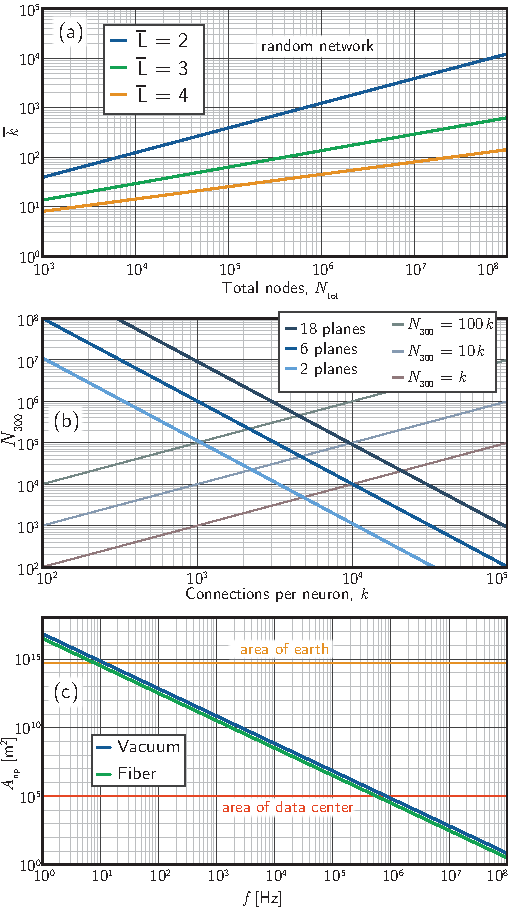
\includegraphics[width=8.6cm]{data_plots.pdf}}
	\captionof{figure}{\label{fig:neuronsOnWafer}Number of neurons on a wafer.}
\end{figure}
%\begin{figure*}[] 
%	\centering{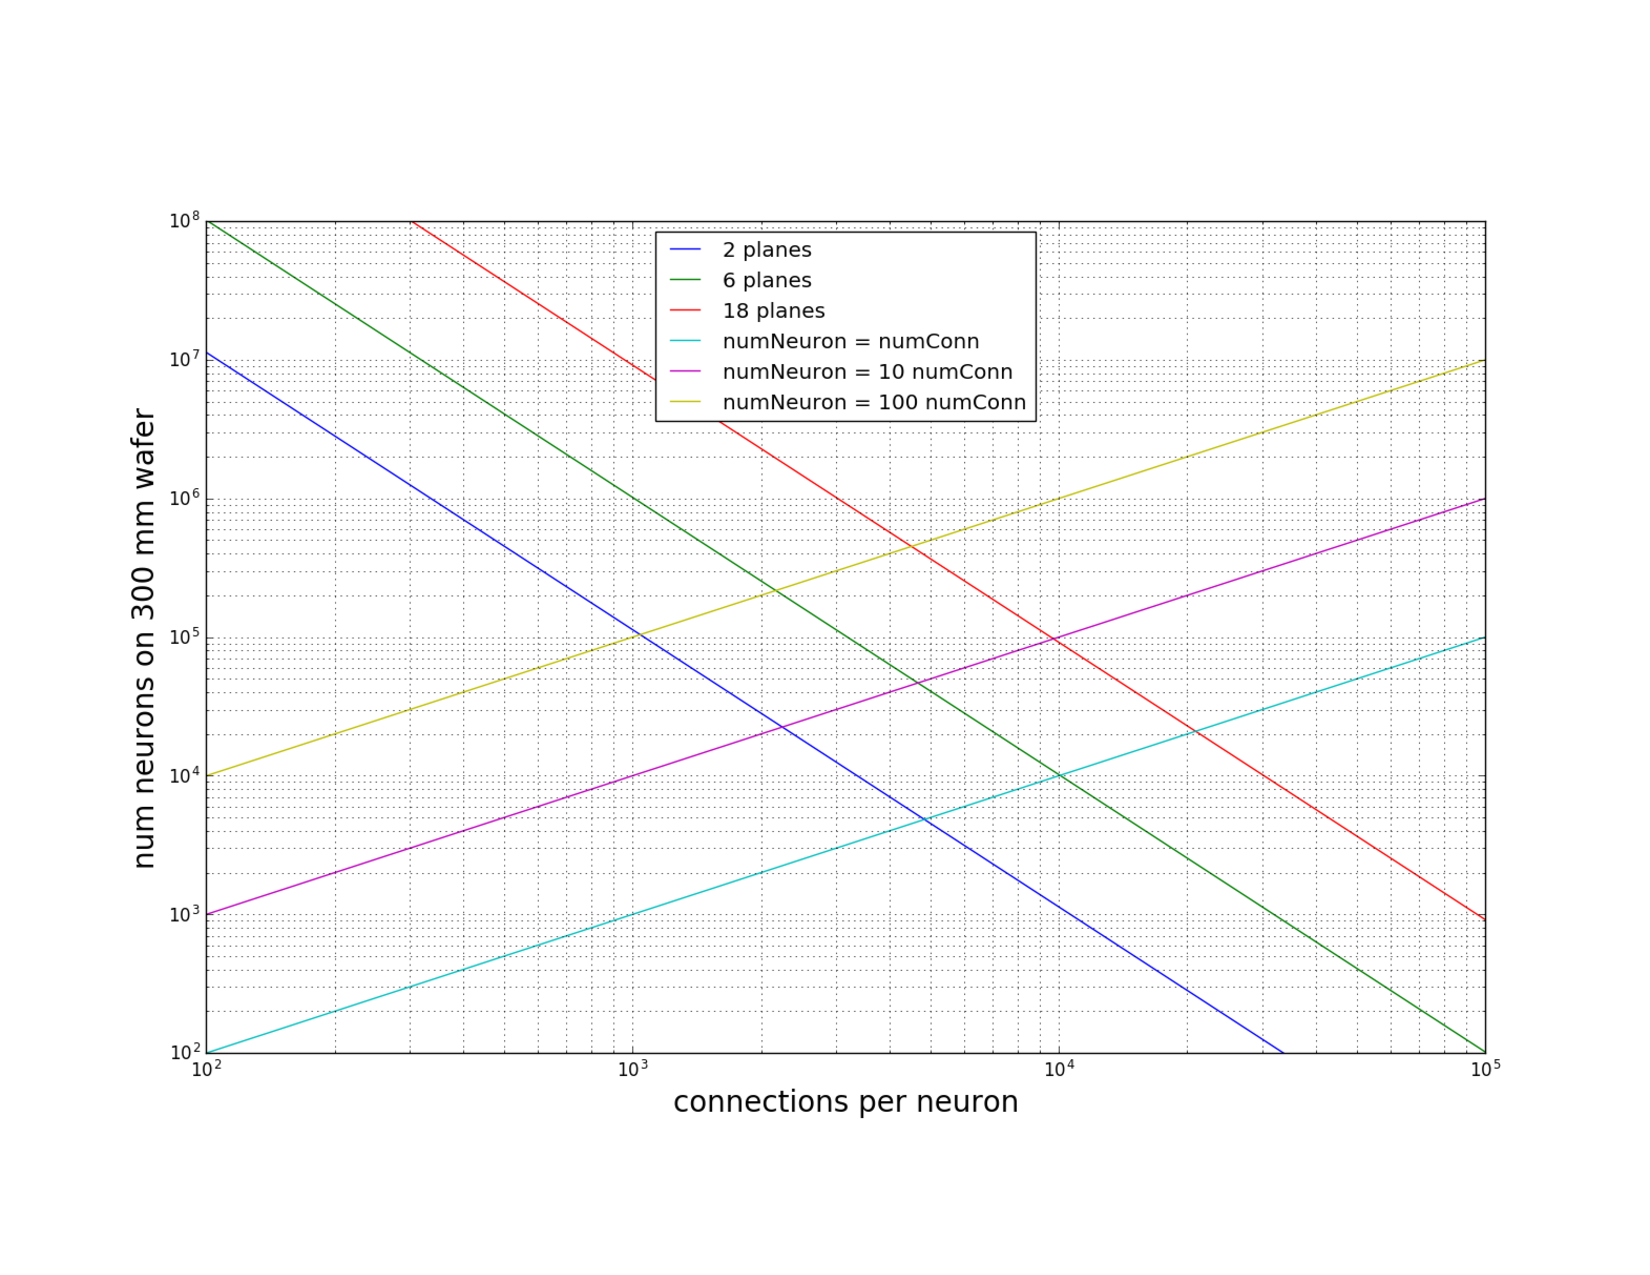
\includegraphics[width=14cm]{neuronsOnWafer.pdf}}
%	\captionof{figure}{\label{fig:neuronsOnWafer}Number of neurons on a wafer.}
%\end{figure*}
This expression is plotted in Fig.\,\ref{fig:neuronsOnWafer}. This estimate informs us that a 300-mm wafer with six waveguide planes can support roughly one million neurons if they each have one thousand connections. As a point of comparison, Ref.\,\cite{kuwa2017} finds that through multi-layer, wafer-scale integration of logic and memory, 250 million electrical neurons could fit on a 300-mm wafer. The trade-off is, of course, speed, as the shared communication network would limit the electrical neurons studied in Ref.\,\ref{kuwa2017} to 10\,Hz operation. Nevertheless, the message of Fig.\,\ref{fig:neuronsOnWafer} is that photonic routing results in large area consumption. If two planes of routing waveguides are used, 100,000 neurons with 1000 connections each can fit on a wafer. With six planes, one million such neurons can fit on a wafer, and with 18 routing planes, the number is close to 10 million. The human cortex contains over 10 billion neurons. An optoelectronic brain larger than a bumble bee will not fit on a wafer.

%\begin{figure*}[] 
%	\centering{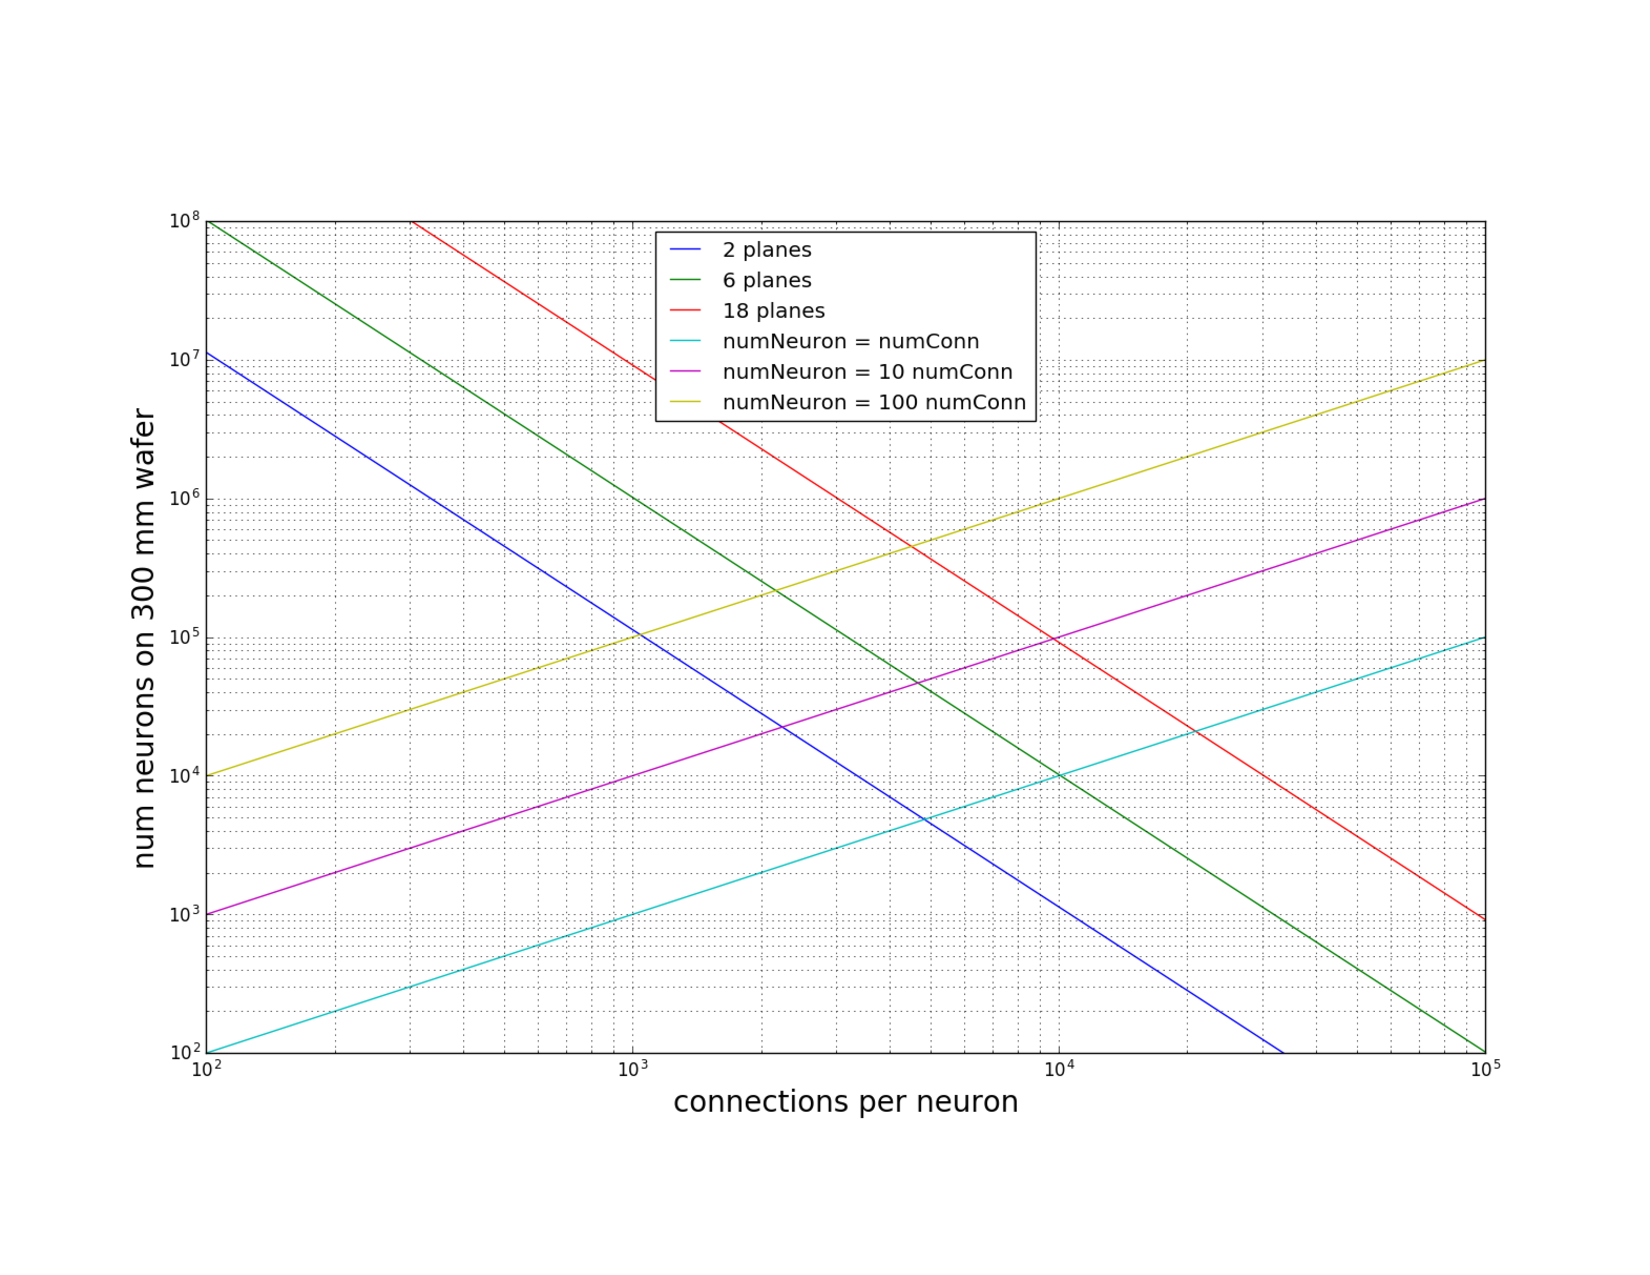
\includegraphics[width=14cm]{communicationScales.pdf}}
%	\captionof{figure}{\label{fig:communicationScales}Photonic interconnection on various length scales.}
%\end{figure*}
Optoelectronic intelligence will require communication between wafers. Wafers can be stacked vertically, and free-space optical links can send photons from a source on one wafer to a detector on a wafer above or below, as illustrated in Fig.\,\ref{fig:communicationScales}(a). Such 3D wafer-stacking techniques are being developed for electronics, but the ability of light to propagate through free space (or liquid helium) and the ten-micron alignment tolerances enabled by wide-area photodetectors \cite{mave2013} make such 3D integration promising for photonic communication as well. Assuming SNSPDs receiving vertical communication have a pitch of 25\,\textmu m, a 300-mm octagon could support $10^8$ vertical communication links between two wafers. Assuming half of this area is for feed-forward communication from the lower wafer to the upper wafer, and half is for feed-back from the upper wafer to the lower wafer. This would result in $5\times10^7$ synaptic connections originating from neurons on one wafer and terminating in neurons on a vertically adjacent wafer. If each wafer had one million neurons with one thousand connections per neuron within the wafer, the total number of intra-wafer synaptic connections would be $10^9$. Therefore, the number of synapses present in a layer of this network that originated on a previous layer would be 5\%, similar to the fraction observed in the laminar structure of biological cortex (Ref.\,\cite{bu2006}, pg. xx).

In addition to free-space vertical coupling, inter-wafer communication can be achieved at wafer edges with in-plane waveguide couplers, as shown in Fig.\,\ref{fig:communicationScales}(c). In the octagonal (truncated square) tiling used here for illustration, each wafer makes such connections to neighbors in the cardinal directions. With a 10\,\textmu m pitch, 11,500 wafer-edge couplers could be supported in each of the cardinal directions with 46,000 total in-plane, lateral connections. Such a system would demonstrate strong connectivity within the vertical stack of the wafers, and weaker lateral connectivity between wafers in the same horizontal plane. Such an architecture resembles the columnar organization of cortex.  

The wafer tiling we have just described leads to a picture of optoelectronic networks with vertically stacked columns of wafers with horizontal connectivity emanating from the perimeter of each wafer. To achieve communication from within these columns to other (perhaps distant) regions of the network, optical fibers are ideal. Within the truncated square tiling under consideration, the square areas at diagonals between wafers can support fiber-optic bundles. These optical fiber tracts are analogous to white matter in the brain. One such region could house a million standard single-mode fibers of 125\,\textmu m diameter. These fibers will emanate from all wafers within the column, so the number of outputs available to each wafer will depend on how many vertically integrated wafers are utilized in a column. If six wafers are stacked in a column, each wafer would have roughly 167,000 output fibers to carry information to distant regions of the network. With one million neurons on a wafer, this would mean not every neuron on the wafer would be able to couple to a fiber for long-distance communication. This again is consistent with brain organization wherein the number of long-distance axons emanating from a region is smaller than the number of neurons within the region. Note, however, that each of these fibers can branch as it propagates through the white matter, so a neuron with access to a single wafer-edge fiber could establish multiple long-range synaptic connections. 

On a wafer, photonic fan-out across dielectric waveguides enables neurons to make thousands of direct connections without the limits of a shared switching network. Free-space and wafer-edge couplers enable significant inter-wafer communication conducive to columnar information processing. Such columns can communicate to one another locally and globally over fiber optic links. With this configuration in mind, we can assess the feasibility of constructing systems on the scale of the human cerebreal cortex, with 10 billion neurons, each with thousands of synaptic connections. If a wafer holds a million neurons, a brain-scale assembly requires 10,000 wafers and would fit in a volume two meters on a side\textemdash the size of a few server racks in a closet. 

Several aspects of this technology make the challenge likely to succeed. First and foremost, due to photonic signaing, it remains possible to achieve efficient communication across the network for systems with orders of magnitude more than 10,000 wafers. Information integration across very large neural systems is physically possible with photonic communication. It also appears practically possible, because all the proposed circuits (for loop neurons and perhaps otherwise) can be fabricated at the wafer scale with existing infrastructure (300\,mm silicon-on-insulator substrates, 193\,nm immersion lithography, equivalent of 45\,nm CMOS node). Ten thousand wafers move through a 45\,nm CMOS foundry every day. If such a foundry were dedicated to fabrication of optoelectronic intelligence, it may be able to produce multiple brain-scale systems per year. Assembly of the wafers into a functional system would be difficult, but probably not more difficult than the construction of a contemporary supercomputer. The requirement of liquid-helium cooling is not a major impediment. The greatest unknown is the light source. If silicon light sources that have already been demonstrated in cryogenic optical links \cite{buch2017} can be produced with internal quantum efficiency $\eta_{\mathrm{qe}}\approx 10^{-3}$, we anticipate this project will be economically viable. At present, $\eta_{\mathrm{qe}} = 5\times10^{-7}$ has been demonstrated in the first attempt with no optimization of optical or electrical properties. These light sources need not achieve high performance. We only require they produce incoherent pulses of 10,000 photons ($\approx 1$\,fJ) at 20\,MHz. If no silicon light source operating at 4\,K can meet these criteria, and integration of III-V light sources on silicon wafers is required, the cost and complexity of a project at this scale may become prohibitive.

\section{\label{sec:discussion}Discussion}
At present, the challenge of creating an artificial intelligence rivaling a human appears formidable with the use of silicon electronics alone. The primary challenge arises because direct signaling between large numbers of neurons is not possible due to the charging requirements of wires and devices, so shared communication infrastructure is required, resulting in a connectivity/speed tradeoff. The use of photonic communication will mitigate this tradeoff, despite the increased size of photonic interconnection networks. Photonic fanout enables direct connections between large numbers of neurons, and the velocity of light enables communication across ten-meter systems before communication limits network speed. 

Light is excellent for communication, while electronics excel at computation. Artificial neural hardware should be designed and constructed to maximally leverage photonic communication while performing synaptic, dendritic, and neuronal functions with electronic circuits for complexity of computation. Superconducting optoelectronic circuits appear to naturally implement these functions, in part because light sources and detectors work much better at low temperature, and in part because of the utility of Josephson nonlinearities for neural computation. The von Neumann architecture emerged to perform arithmetic calculations in a manner based on a Turing machine. Neural information processing departs markedly from the sequential operation of a Turing apparatus, so we should not be surprised that optimal hardware may differ. Yet for the superconducting optoelectronic hardware discussed here, the fabrication infrastructure is largely the same as contemporary CMOS. The construction, facilities, and cost of a brain-scale optoelectronic system are likely comparable to a contemporary supercomputer. Understanding the principles of network information processing and designing the architecture to achieve general intelligence are the true grand challenges.

So what are the next steps to realize this technology? Low-cost source-detector integration at the wafer scale is required. These active devices must be augmented with improvements in deposited dielectrics photonic routing enabling more planes with lower loss. For system scaling, improved fiber-to-waveguide coupling and multi-wafer modules must be demonstrated. All the hardware improvements will not lead to AGI without further theoretical analysis at the device, circuit, and system levels. As is the case with other artificial neural systems, theoretical analysis is required to understand how to use these systems, train them, and make them intelligent.

\bibliography{light_in_neural_systems}

\end{document}